\documentclass[../main.tex]{subfiles}

\makeatletter
\@ifundefined{fromRoot}{%
  \newcommand{\fromRoot}[1]{../#1}
  
 % \usepackage{xr}
  % \externaldocument{../main}
}{}

\def\input@path{{\subfix{../}}}
%or: \def\input@path{{/path/to/folder/}{/path/to/other/folder/}}
\makeatother

\graphicspath{
  {\subfix{../}}
  {\subfix{./figures}}
  {\subfix{../figures}}
  {\subfix{./figures/logos-thesis/}}
  {\subfix{../figures/logos-thesis/}}
  {\subfix{./figures/rtexps-pics/}}
  {\subfix{../figures/rtexps-pics/}}
}

\hypersetup{
    pdfauthor   = {Camille MONIÈRE},
    pdftitle    = {Th\`{e}se (Présentation: implémentations)},
    pdfsubject  = {Th\`{e}se (Présentation: implémentations)},
%    pdfkeywords = {mots-cl\'{e}s},
}

\begin{document}

\section{Étude et exploitation du parallélisme}

\subsection{Rappel : Différents niveaux de parallélismes}

\begin{frame}{\acrfull{simd}}
  \begin{columns}
    \begin{column}{.3\linewidth}
      \centering
      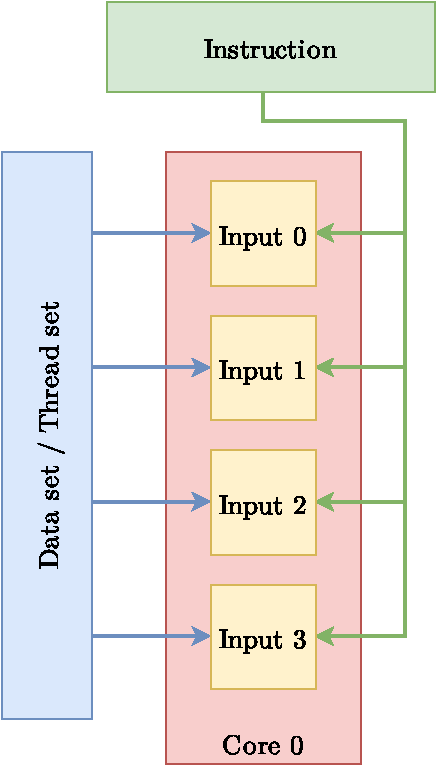
\includegraphics[
        width=\linewidth,
        height=.75\textheight,
        keepaspectratio=true
      ]{figures/drawiopdf/simd_simt.drawio.pdf}
      \captionof{figure}{SIMD en schéma {\tiny --- \itshape UC : Unité de Calcul}}
    \end{column}
    \begin{column}{.7\linewidth}
      \begin{ctrlitemize}{.5 em}
        \item Parallélisme de plus bas niveau.
        \item Consiste en l'exécution d'une même instruction sur plusieurs données.
        \item Une instruction sur $\alpha$ entrées conduit à une accélération d'un facteur $\alpha$.
      \end{ctrlitemize}

      \vspace{2 em}

      \begin{ctrlitemize}{.5 em}
        \item Requiert une unique unité de calcul équipée d'opérateurs adaptés.
        \item Applicable \textbf{uniquement} pour des calculs \textbf{identiques} sur des données \textbf{alignées}.
      \end{ctrlitemize}
    \end{column}
  \end{columns}
\end{frame}


\begin{frame}[fragile]{\acrshort{simd} : Exemple}
  \vspace{- 1 em}
  \begin{columns}
    \begin{column}{.5\linewidth}
      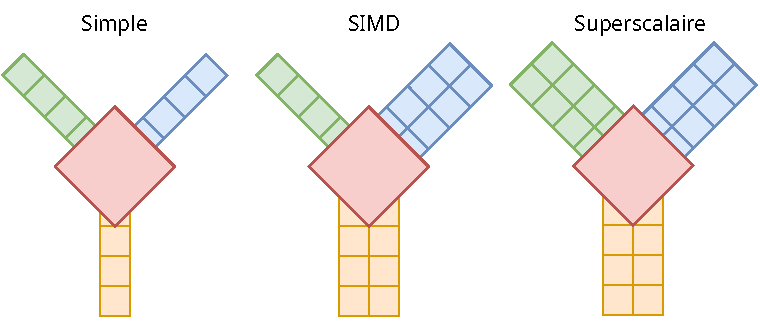
\includegraphics[width=\linewidth]{figures/drawiopdf/testyolo-jm2.pdf}
    \end{column}
    \begin{column}{.5\linewidth}
      Exemple : \\
      \hspace{2 em} \centering Somme termes à termes de $\vect{a} = [a_0, a_1, a_2, a_3]$ et $\vect{b} = [b_0, b_1, b_2, b_3]$ stocké dans $\vect{c} =  [c_0, c_1, c_2, c_3]$ 
    \end{column}
  \end{columns} \vspace{1 em} 

  \begin{columns}
    \begin{column}{.5\linewidth}
      \begin{overlayarea}{\linewidth}{.4\textheight}
        \underline{Séquentiellement ($\thickapprox 4$ instructions)} \vspace{1 em}

        Pour chaque $x$ dans $[0,1,2,3]$, faire :\\
        \hspace{2 em} $c_x = a_x + b_x$

        % \begin{columns}
        %   \begin{column}{.45\linewidth}
        \begin{lstlisting}[title={Sequentiellement en C},style=cstyle,basicstyle=\scriptsize]
 //  a, b et c => double[4]
 for (int i = 0; i < 4; i++) {
   c[i] = a[i] + b[i]; 
 }\end{lstlisting}
        % \end{column}
        % \begin{column}{.5\linewidth}

        %   \begin{lstlisting}[title={Sequentiellement en MATLAB},style=cstyle,language=MATLAB,basicstyle=\tiny]
        %  % a, b, et c => size = (1, 4)
        %  for i in 1 : 4
        %    c(i) = a(i) + b(i)
        %  end\end{lstlisting}
        %          
        %  \end{column}
        % \end{columns}
      \end{overlayarea}
    \end{column}
    \begin{column}{.45\linewidth}
      \begin{overlayarea}{\linewidth}{.4\textheight}
        \underline{En parallèle (SIMD) ($\thickapprox 1$ instruction)} \vspace{1 em}

        $\vect{c} = \vect{a} + \vect{b}$ \\
        \phantom{$c_x$}

        % \begin{columns}
        %   \begin{column}{.5\linewidth}
        \begin{lstlisting}[title={SIMD en C (Intel, double $64$-bit)},style=cstyle,basicstyle=\scriptsize]
 //  a, b et c => double[4]
 c = _mm256_add_pd(a, b);\end{lstlisting}
        % \end{column}
        %           \begin{column}{.5\linewidth}
        %             % \begin{noindent}
%             \begin{lstlisting}[title={SIMD en MATLAB},style=cstyle,language=MATLAB,basicstyle=\tiny]
% % a, b, et c => size = (1, 4)
% c = a + b;\end{lstlisting}
%             % \end{noindent}
        %           \end{column}
        % \end{columns}
      \end{overlayarea}
    \end{column}
  \end{columns}
  \note{
    \begin{itemize}
      \item Les CPU today, c'est cool
      \item Faut leur parler bien
      \item Exemple
    \end{itemize}
  }
\end{frame}

\begin{frame}{Single Program Multiple Data (SPMD)}
  \begin{columns}
    \begin{column}{.4\linewidth}
      \centering
      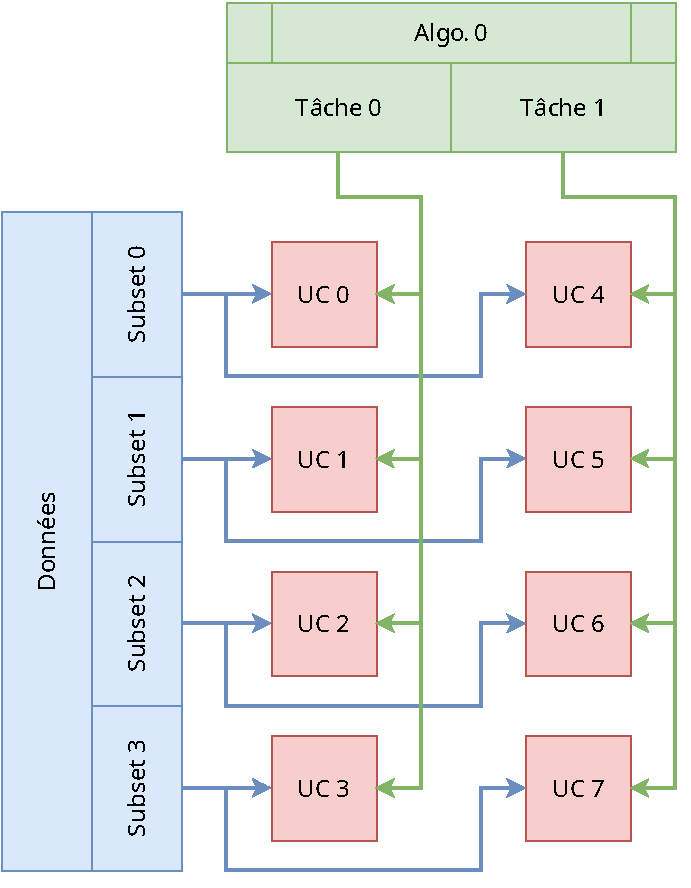
\includegraphics[
        width=\linewidth,
        height=.7\textheight,
        keepaspectratio=true
      ]{figures/drawiopdf/spmd.drawio.pdf}
      \captionof{figure}{SPMD en schéma {\tiny --- \itshape UC : Unité de Calcul}}
    \end{column}
    \begin{column}{.6\linewidth}
      \begin{ctrlitemize}{.5 em}
        \item Parallélisme de type \emph{Multiple Instructions Multiple Data (MIMD)}.
        \item Consiste à segmenter un processus ou algorithme en sous-tâches travaillant indépendamment sur des sous-ensembles de données.
      \end{ctrlitemize}

      \vspace{1.4 em}

      \begin{ctrlitemize}{.5 em}
        \item Accélération fortement dépendante du degré d'indépendance des sous-tâches.
        \item Le temps de répartition des calculs et données aux UCs n'est pas négligeable \cite{hillAmdahlLawMulticore2008}.
      \end{ctrlitemize}
    \end{column}
  \end{columns}
  \blfootnote{\textcite{hillAmdahlLawMulticore2008}}
  \note{
    Lis $+$ dis boost débit mais attention latence !
  }
\end{frame}

\begin{frame}{SPMD : Exemple --- Somme de $10^9$ valeurs}
  \begin{columns}
    \begin{column}{.33\linewidth}
      \begin{overlayarea}{\linewidth}{.85\textheight}
        \centering
        \textbf{Séquentielle (1 thread)} \vspace{.03\textheight}

        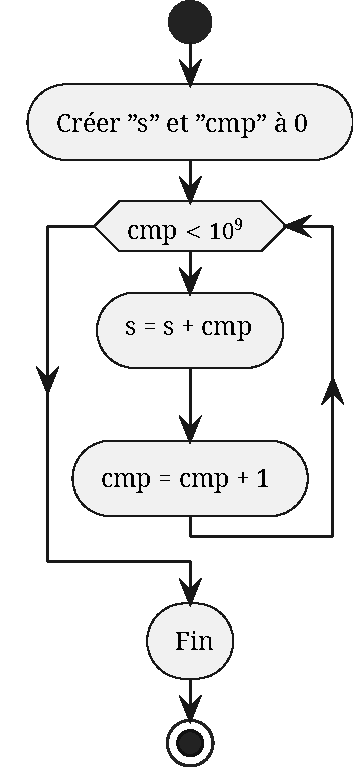
\includegraphics[
          width=\linewidth,
          height=.45\textheight,
          keepaspectratio=true,
        ]{figures/drawiopdf/sum_seq.pdf} \vspace{1em} 

        $T_{seq} = T_{iter} \times 10^9$ \\
        VS
        $T_{//}  = \frac{T_{seq}}{4} + T_{start} + T_{stop} + 4 \times T_{iter}$ \\
      \end{overlayarea}
    \end{column}
    \begin{column}{.66\linewidth}
      \begin{overlayarea}{\linewidth}{.85\textheight}
        \centering
        \textbf{Parallèle (4 threads)} \vspace{.03\textheight}

        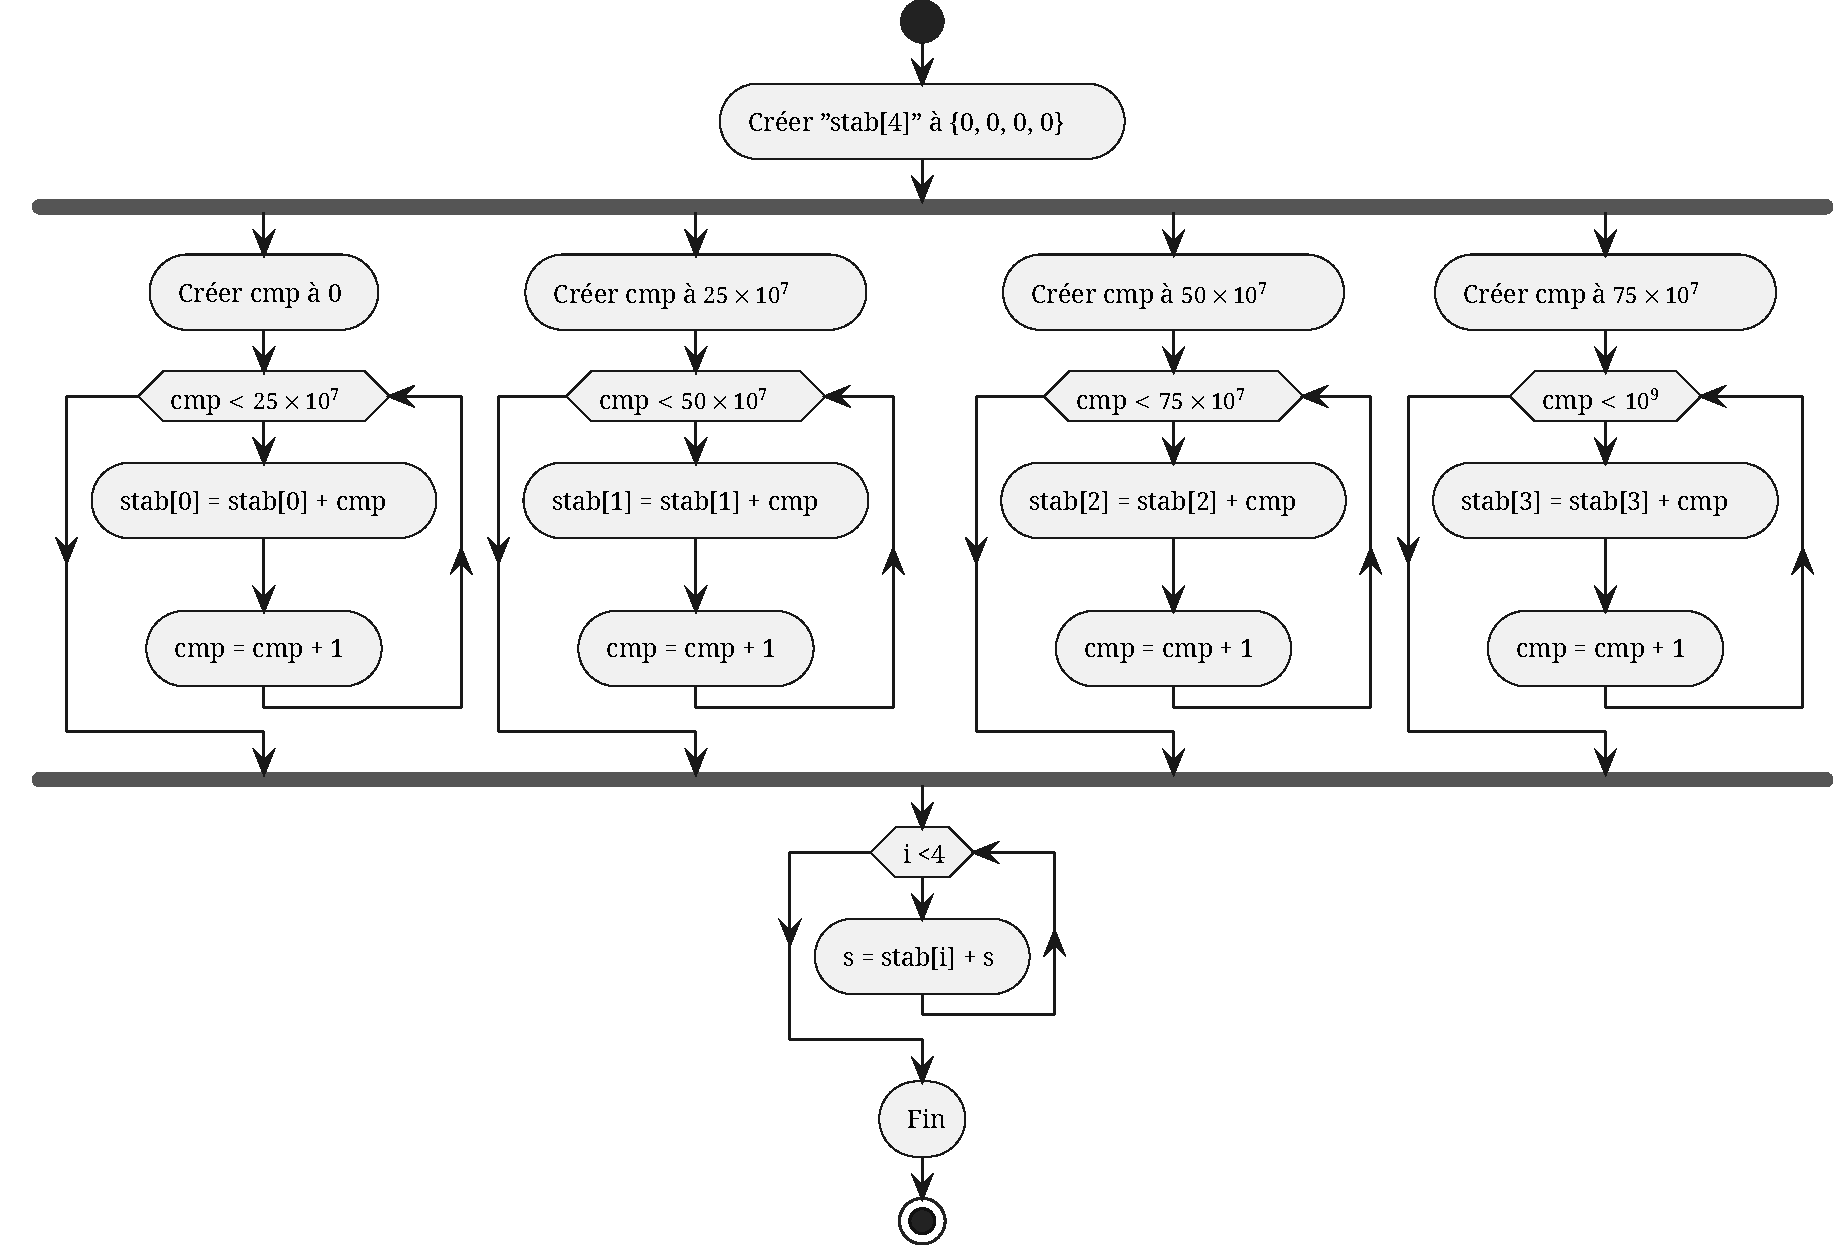
\includegraphics[
          width=\linewidth,
          height=.8\textheight,
          keepaspectratio=true,
        ]{figures/drawiopdf/sum_parallel.pdf}
      \end{overlayarea}
    \end{column}
  \end{columns}
\end{frame}

\begin{frame}{Multiple Programs Multiple Data (MPMD)}
  \begin{columns}
    \begin{column}{.5\linewidth}
      \centering
      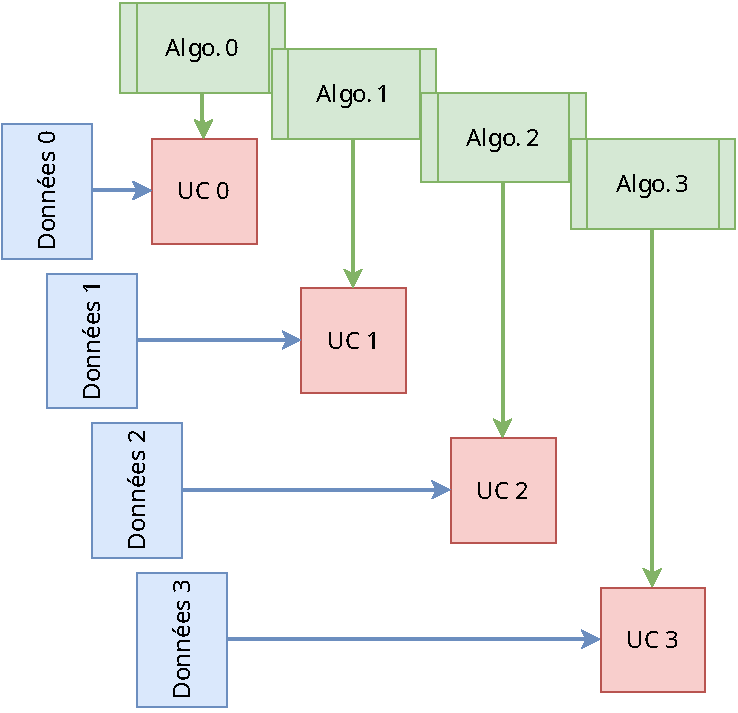
\includegraphics[
        width=\linewidth,
        height=.75\textheight,
        keepaspectratio=true
      ]{figures/drawiopdf/mpmd.drawio.pdf}
      \captionof{figure}{MPMD en schéma {\tiny --- \itshape UC : Unité de Calcul}}
    \end{column}
    \begin{column}{.5\linewidth}
      \begin{ctrlitemize}{.5 em}
        \item Parallélisme de plus haut niveau et de type \emph{MIMD}.
        \item Consiste à segmenter un programme en plusieurs processus ou algorithmes, aussi indépendants que possible.
      \end{ctrlitemize}

      \vspace{1.4 em}

      \begin{ctrlitemize}{.5 em}
        \item À nouveau, accélération fortement dépendante du degré d'indépendance des algorithmes.
      \end{ctrlitemize}
    \end{column}
  \end{columns}
  \note{
    Lis $+$ dis gain latence mais debit limité par plus lent !
  }
\end{frame}

\begin{frame}{MPMD : Exemple --- Chaine de communication}
  \begin{center}
    \includegraphics[
      width=\linewidth,
      height=.35\textheight,
      keepaspectratio=true
    ]{figures/tikzpicture/chain_mpmd.pdf}
    \captionof{figure}{Répartition des tâches de réception sur plusieurs unités de calcul.}
  \end{center}

  \vspace{1 em}

  \begin{columns}
    \begin{column}{.5\linewidth}
      Le débit total est contraint par :
      \begin{itemize}
        \item Les transferts de données ;
        \item Le débit de la tâche la plus lente.
      \end{itemize}
    \end{column}
  \end{columns}
  \note{
    Lis $+$ ui ui on pourrait mixer
  }
\end{frame}

\begin{frame}
  \frametitle{En tirer parti}

  \begin{columns}
    \begin{column}{.5\linewidth}
      \begin{overlayarea}{\linewidth}{.85\textheight}
        \centering
        \textbf{\large \underline{\phantom{g}Logiciel\phantom{g}}} \vspace{.25 em}

        \begin{ctrlitemize}{.5 em}
          \item Limité par l'architecture du processeur.
          \item Effort d'adaptation de la description algorithmique à l'architecture \cite{armNEONProgrammerGuide2013,intelrArchitectureInstructionSet2022} \textbf{et} au langage utilisé (C/\cpp{}, Python, MATLAB \dots)
          \item []
        \end{ctrlitemize}

        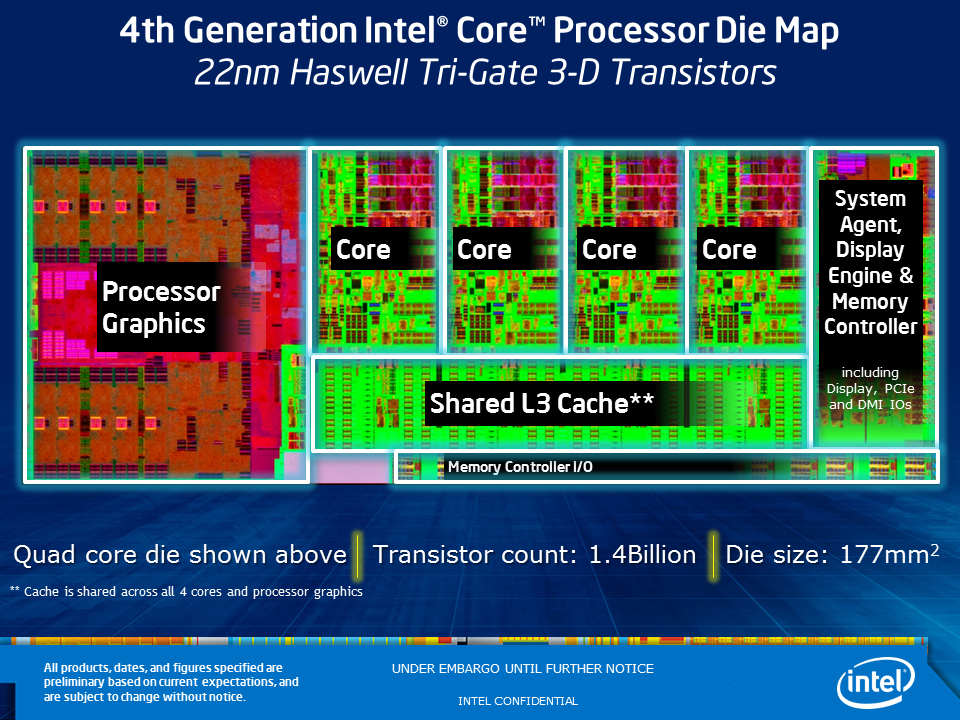
\includegraphics[
          width=\linewidth,
          height=.2\textheight,
          keepaspectratio=true,
          clip,
          trim = {15px 227px 15px 140px},
        ]{figures/processor-2217771_1920.jpg}
        \captionof{figure}{Schéma d'implémentation d'un Intel\textregistered{} Core\texttrademark{} 4th gen, \textrm{\tiny par Intel, CC-BY-SA, flikr.com}}
      \end{overlayarea}
    \end{column}
    \begin{column}{.5\linewidth}
      \begin{overlayarea}{\linewidth}{.85\textheight}
        \centering
        \textbf{\large \underline{\phantom{g}Matériel\phantom{g}}} \vspace{.25 em}

        \begin{ctrlitemize}{.25 em}
          \item Grande liberté, les UCs étant définies par le concepteur lui-même.
          \item Temps de conception notablement plus long qu'en logiciel.
          \item Limité par les ressources de calculs disponibles (LUT, Flip-Flop, DSP).
          % \item []
        \end{ctrlitemize}

        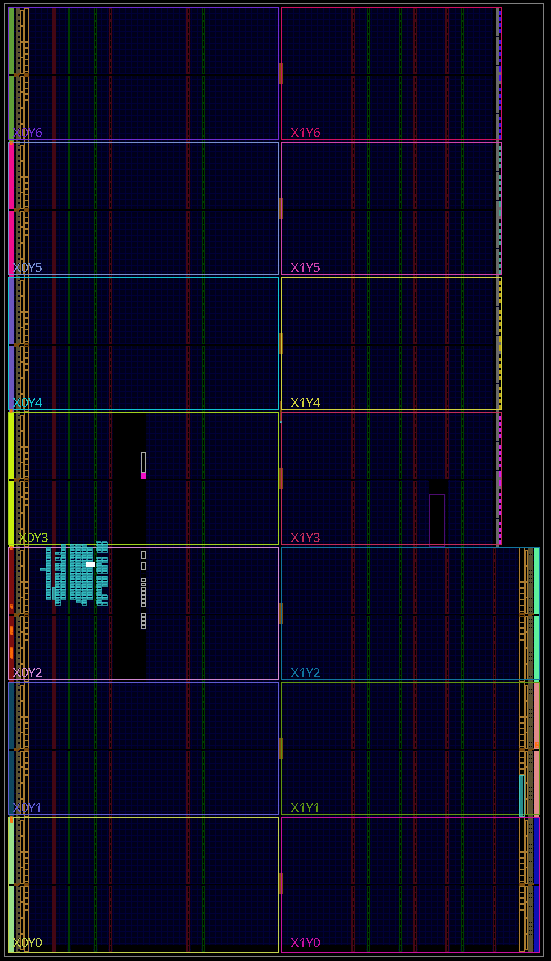
\includegraphics[
          width=.25\textheight,
          height=\linewidth,
          keepaspectratio=true,
          angle = 90,
        ]{figures/xilinxkintex7_20221229_154930.png}
        \captionof{figure}{Schéma d'implémentation d'un Kintex\texttrademark-7 de Xilinx\textregistered, \textrm{\tiny par Xilinx, Tous droits réservés}}
      \end{overlayarea}
    \end{column}
  \end{columns}
  \blfootnote{\textcite{armNEONProgrammerGuide2013,intelrArchitectureInstructionSet2022}}
  \note {
    Déroule juste, on verra après
  }
\end{frame}

\subsection{Adaptation aux corrélations}

\begin{frame}{En logiciel --- FFT}
  \begin{columns}
    \begin{column}{.4\linewidth} \centering
      \includegraphics[
        width=\linewidth,
        height=.45\textheight,
        keepaspectratio=true,
      ]{figures/tikzpicture/grid_fft_paral.pdf}
    \end{column}
    \begin{column}{.5 \linewidth}
      \centering
      \includegraphics[
        width=\linewidth,
        height=.45\textheight,
        keepaspectratio=true,
      ]{figures/tikzpicture/corr_method_fftshar_stdl.pdf}
    \end{column}
  \end{columns}
  \begin{columns}
    \begin{column}{.9\linewidth} \centering
      \begin{itemize}
        \item Stratégie ``SPMD'' selon l'axe \textcolor{Red}{$//_{\Delta}$} :
              \begin{itemize}
                \item un thread de calcul par hypothèse temporelle,
                \item lancement de la procédure tous les $q$ chips.
              \end{itemize}
        \item L'axe \textcolor{Blue}{$//_{\omega}$} reste séquentiel, le coût de la parallélisation s'est avéré trop important.
        \item Les FFTs proviennent de FFTW3 \cite{frigoDesignImplementationFFTW32005a}, et donc utilisent, entres autres, du ``SIMD''.
      \end{itemize}
    \end{column}
  \end{columns}
  \blfootnote{\textcite{frigoDesignImplementationFFTW32005a}}
\end{frame}

\begin{frame}{En logiciel --- Time Sliding}
  \begin{columns}
    \begin{column}{.4\linewidth} \centering
      \includegraphics[
        width=\linewidth,
        height=.45\textheight,
        keepaspectratio=true,
      ]{figures/tikzpicture/grid_fft_paral.pdf}
    \end{column}
    \begin{column}{.5 \linewidth}
      \centering
      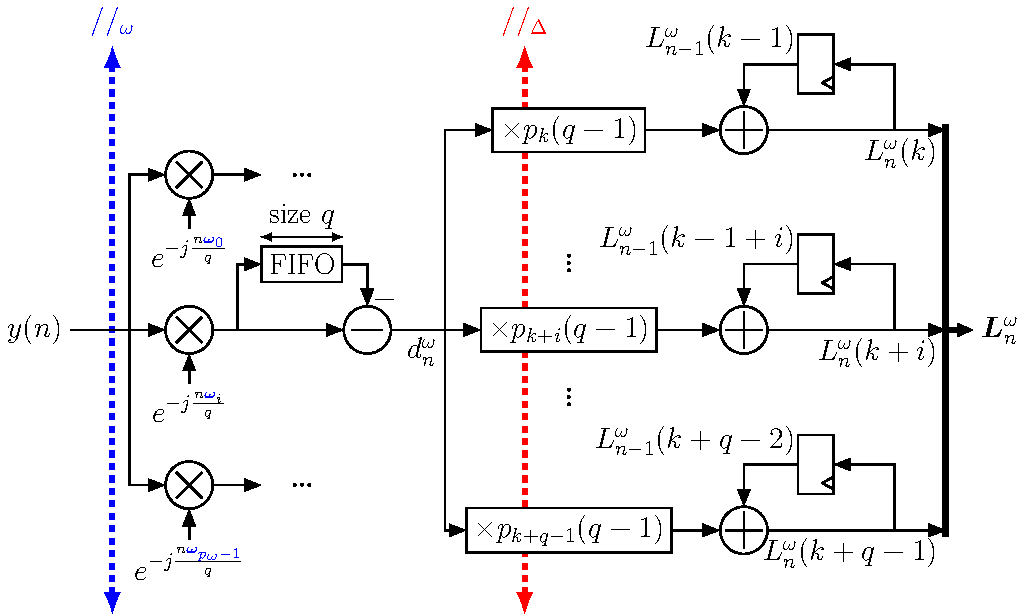
\includegraphics[
        width=\linewidth,
        height=.45\textheight,
        keepaspectratio=true,
      ]{figures/tikzpicture/corr_method_subts_stdl.pdf}
    \end{column}
  \end{columns}
  \begin{columns}
    \begin{column}{.9\linewidth} \centering
      \begin{itemize}
        \item Utilisation de la version ``index shift'', plus performantes.
        \item Stratégie ``SIMD'' selon l'axe \textcolor{Red}{$//_{\Delta}$} :
              \begin{itemize}
                \item décomposition des calculs dans l'espace des réels,
                \item description algorithmique telle que le compilateur puisse la vectoriser.
              \end{itemize}
        \item Comme pour la FFT, l'axe \textcolor{Blue}{$//_{\omega}$} reste séquentiel.
      \end{itemize}
    \end{column}
  \end{columns}
  \blfootnote{\textcite{frigoDesignImplementationFFTW32005a}}
\end{frame}

\begin{frame}{En matériel}
  \begin{columns}
    \begin{column}{.45\linewidth}
      \centering
      \begin{overlayarea}{\linewidth}{.65\textheight}
        \underline{\textbf{FFT}}
        \begin{ctrlitemize}{1 em}
          \item Parallélisation MASSIVE de modules FFT optimisés ;
          \item Impose une forte contrainte sur les ressources matérielles ;
          \item Non concluant à l'heure actuelle \dots
        \end{ctrlitemize}
      \end{overlayarea}
    \end{column}
    \begin{column}{.45\linewidth}
      \centering
      \begin{overlayarea}{\linewidth}{.65\textheight}
        \underline{\textbf{Time Sliding}}
        \begin{ctrlitemize}{1 em}
          \item Utilisation de la version ``index shift'' à nouveau ;
          \item Parallélisation complète des opérateurs, $\textcolor{Red}{\mpd{}} \times \textcolor{Blue}{\mpo{}}$ calculés en parallèle ;
          \item En cours de finalisation.
        \end{ctrlitemize}
      \end{overlayarea}
    \end{column}
  \end{columns}

  % \begin{columns}
  %   \begin{column}{.8\linewidth}
  %     \centering
  %       \begin{overlayarea}{\linewidth}{.1\textheight}
  %         {\small Note : utilisation de la synthèse de haut-niveau (HLS) pour convertir des descriptions comportementales en architectures matérielles.}
  %     \end{overlayarea}
  %   \end{column}
  % \end{columns}
  \only<2>{
    \vspace{1 em}
    
    \centering \Huge En cours !
  }
  \note{
    En cours, ingénieure L. Volpin supervisée, à récupérer 
  }
\end{frame}

\begin{frame}{Résultats d'implémentation}{Débits binaires d'information fonction de \textcolor{Red}{\pd{}}, pour \textcolor{Blue}{$\mpo{} = 4$}}
  \begin{columns}
    \begin{column}{.5\linewidth}
      \begin{overlayarea}{\linewidth}{.75\textheight}
        \centering
        \includegraphics[height = .65 \textheight]{figures/pgfplots/results_implem_through_intel.pdf}
        \captionof{figure}{Plateforme Intel\textregistered{} x86\_64, $40$ cœurs Xeon\texttrademark{}-6148,\\horloge à $2,8$ GHz.}
      \end{overlayarea}
    \end{column}
    \begin{column}{.5\linewidth}
      \begin{overlayarea}{\linewidth}{.75\textheight}
        \centering
        \includegraphics[height = .65 \textheight]{figures/pgfplots/results_implem_through_jetson.pdf}
        \captionof{figure}{Plateforme ARM\textregistered{}, $12$ cœurs Cortex\texttrademark{}-A78AE,\\horloge à $2,2$ GHz.}
      \end{overlayarea}
    \end{column}
  \end{columns}

\end{frame}

\begin{frame}{Résultats d'implémentation}{Consommations énergétiques fonction de \textcolor{Red}{\pd{}}, pour \textcolor{Blue}{$\mpo{} = 4$}}
  \begin{columns}
    \begin{column}{.5\linewidth}
      \begin{overlayarea}{\linewidth}{.75\textheight}
        \centering
        \includegraphics[height = .65 \textheight]{figures/pgfplots/results_implem_nrj_intel.pdf}
        \captionof{figure}{Plateforme Intel\textregistered{} x86\_64, $40$ cœurs Xeon\texttrademark{}-6148,\\horloge à $2,8$ GHz.}
      \end{overlayarea}
    \end{column}
    \begin{column}{.5\linewidth}
      \begin{overlayarea}{\linewidth}{.75\textheight}
        \centering
        \includegraphics[height = .65 \textheight]{figures/pgfplots/results_implem_nrj_jetson.pdf}
        \captionof{figure}{Plateforme ARM\textregistered{}, $12$ cœurs Cortex\texttrademark{}-A78AE,\\horloge à $2,2$ GHz.}
      \end{overlayarea}
    \end{column}
  \end{columns}

\end{frame}

\end{document}
